\documentclass[12pt]{report}
\pagestyle{empty}
\usepackage[margin = 1in]{geometry}
\usepackage{array}
\usepackage{amsmath}
\usepackage{caption}
\usepackage{subcaption}
\usepackage{amsfonts}
\usepackage{enumerate}
\usepackage{graphicx}
\usepackage{float}


\newcolumntype{M}{>{$}c<{$}}
\setlength{\parindent}{0mm}
\newcommand{\tab}{\hspace*{2em}}
\renewcommand*{\arraystretch}{1.5}
\newcommand{\comment}[1]{}

\title{A Stochastic Spatial Model for Tumor Growth}
\author{Aashiq Dheeraj, Mentor: Rick Durrett}

\begin{document}
\maketitle

\chapter*{Acknowledgements}
This research was conducted under the supervision of Prof. Richard Durrett (Duke University), and was supported, in part, by the National Science Foundation through Research Training Group grant DMS-0943760 to the Department of Mathematics at
Duke University
\newpage

\chapter*{Abstract}
Evolutionary game theory can be used to study the interactions of different cell phenotypes and describe tumor population dynamics. Instead of killing tumor cells, clinical treatment could aim to change the nature of the evolutionary game-- enabling healthy cells to outcompete malignant cells. Most applications of  evolutionary game theory to tumor growth have considered the tumor as a homogeneously mixing population that is governed by the replicator equation. We model the tumor population as an interacting particle system (IPS), with discrete individuals, stochastic local interactions, and explicit spatial consideration. Using this model, we see how predictions are changed when space is taken into account. In particular, we consider the analysis of multiple myelomas proposed by Dingli \cite{Dingli2009} and Basanta's work on glioma progression \cite{Basanta2008}. Our model agrees with Basanta's in that we should have coexistence between the three tumor phenotypes, but the spatial model allows coexistence in a significantly wider region of parameter space. Dingli's tumor population exhibits bistability in a certain parameter regime. Our spatial model predicts a transition between the two stable states at a critical parameter value, so there is no bistability. 

\chapter*{Introduction}
	The theory of evolutionary games was introduced to study ecological competitions \cite{Smith1986}. However 15 years ago, Tomlinson suggested that it could be used to study interactions between tumour cells \cite{Tomlinson1997,TomBod}. More recently, Axelrod, Axelrod, and Pienta  \cite{Axelrod2006} have explained how the cooperation of cancer and normal cells can bring on mutually beneficial events such as angiogenesis (the development of blood vessels), Dingli et al (2009) have studied the interactions between osteoclast, osteoblasts, and tumor cells in multiple myeloma, and in a series of papers Basanta and coauthors have studied the role of glycolysis in glioma progression and invasion \cite{Basanta2008,Basanta2011}. \\
	
	
	All of these analyses assume that the population of cells is homogeneously mixing while in reality, each cells compete only with those nearby. Durrett and Levin \cite{Durrett1994} show that the introduction of explicit spatial considerations can change the qualitative behavior of a game. They consider four different approaches to modeling evolutionary games. The mean field approach assumes that every individual interacts with every other with equal probability. This assumption gives the benefit of often analytically tractable ODE models. Patch models group individuals into homogeneously mixing patches, with possible migration in between, but no other spatial structure. Reaction-diffusion equations have individuals as continuous concentrations that can diffuse through space and interact only locally. Finally, interacting particle systems have discrete  individuals and treat space explicitly. There are some interesting analytical results that reduce an interacting particle system to a limiting reaction-diffusion equation. Here, we will consider an IPS model for several games, comparing the results to those of earlier mean-field models. \\
	
	
	
	
	

	
\chapter*{Materials and Methods}
\section*{Game Theoretic Model}
	In evolutionary game theory, it is common to use an ODE model based on pairwise interactions. Suppose that we have $n$ cell types. Let $x_i$ denote the fraction of the population that is cell type $i$. We must have $\sum_{i=1}^n x_i = 1$. Then, the state of the population, $\vec{x}$ can be represented as a point on the $n$-dimensional simplex. 
	
	The time-evolution of this state is given by the replicator equation. For each $i$, 
	$$\dot{x_i} = x_i (W_i(\vec{x}) - \overline{W})$$
	
	where $W_i$ is the fitness of cell type $i$ and $\overline{W}$ is the average fitness. Suppose that the fitness payoff due to the interaction between cell types depends linearly on the cell proportions. We can write a payoff matrix, U, that captures the results of this interaction. Then $W_i(\vec{x}) = \vec{\textbf{e}}_i \cdot G\vec{x} $ and $\overline{W} = \vec{x}^\top G \vec{x}$.
	
\section*{Spatial Refinement}

According to this model, the fitness of a given individual depends upon the state of the population as a whole. However, when individuals are distributed in space, this fitness should only depend upon interactions with nearby neighbors. If the population is homogeneously mixing, all sites are neighbors. The replicator equation can then be viewed as a mean-field approximation to a spatial game. As shown by Durrett and Levine, including spatial effects can have important implications for the dynamics \cite{Durrett1994}.\\

In our model, cells are represented as points on the lattice $\mathbb{Z}^d$, initialized to one phenotype. The "neighborhood" of a given cell refers to the von Neumann neighborhood. In 3 dimensions, this consists of the consisting of the 3-6 cells with which it shares a face. The "fitness" of a given cell is computed by summing over the payoffs for interactions with each neighbor. The payoffs are taken from the payoff matrix for the particular game under consideration. The time-evolution of the lattice is given by choosing a cell at random and replacing it with one of its neighbors, chosen with probability proportional to fitness.
\begin{figure}
\centering
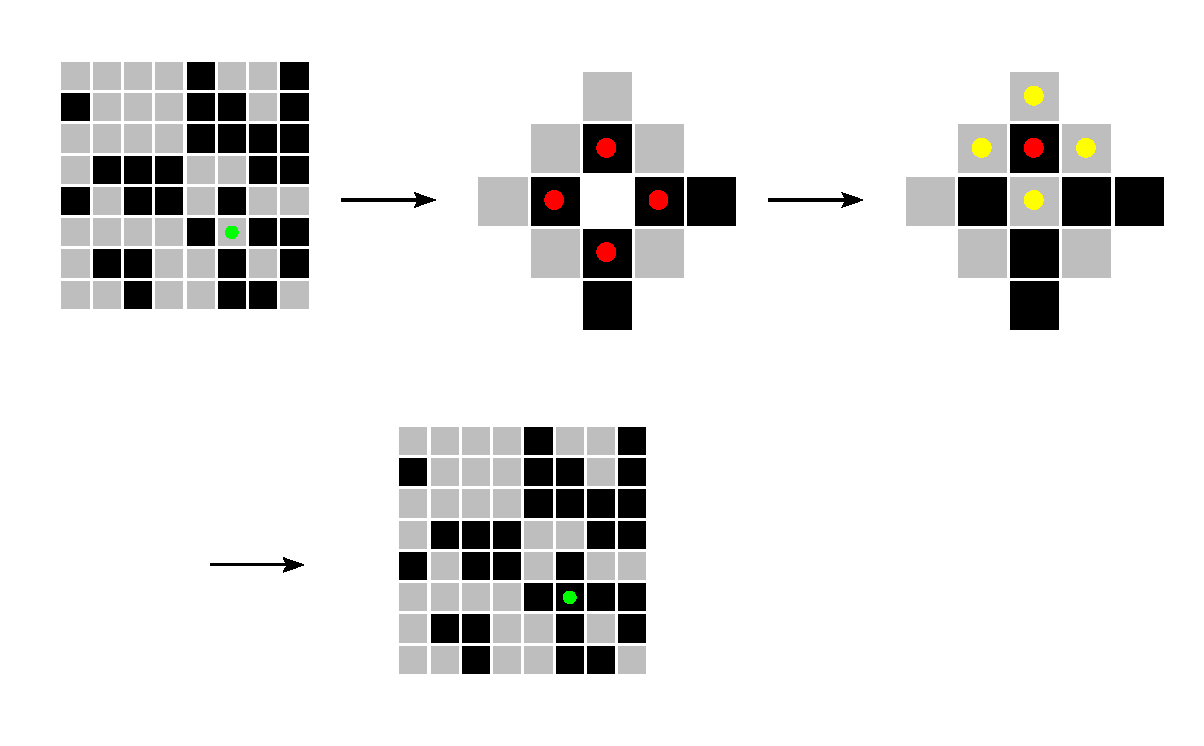
\includegraphics[width = \linewidth]{Diagrams/General/themodel}
\caption{An example of a Moran update. The cell marked green is randomly selected to die. The fitness of each red neighbor is computed using its yellow neighbors (including the dead cell). Finally, the update is made.}
\end{figure}

There are a few metrics one can use to characterize the behavior of our model. A good way to show coexistence is to look at cell type frequencies over time. If they are stable over long periods of time or have sustained oscillations, this might indicate coexistence. The lattice used must be large enough that stochastic fluctuations in population do not accidentally eliminate a cell type, in which case the predicted dynamics could be far off. As long as this is satisfied, the initial conditions should not matter. This is true of stochastic models as discussed in Durrett and Levin \cite{Durrett1994}, which have infinite size. The dynamics of interest tend to take place at a characteristic length scale, so the lattice we use must be large enough to capture them. To determine this, we need a metric to quantify the size of the structures we observe in the spatial model. We define the degree of clustering as the ratio of identical neighbor pairs to total neighbor pairs. If the clustering tends to keep increasing, this might indicate that the chosen lattice is  not large enough.\\

After some trial and error, we settled on a lattice of size 75 x 75 x 75 with periodic boundary conditions (torus). Around this size, the clustering statistic for simulations that exhibit coexistence is steady well below 1. In smaller simulations, the clustering statistic goes to 1 and the output is noisier. Initially, simulations were run in 2 dimensions, but the model was poorly  as the voter model has no unique stationary distribution in 2 dimensions.\\

One can arrive at analytical results for two-strategy games by considering voter model perturbations. Cox, Durrett, and Perkins consider the limiting reaction diffusion equations that arise from perturbations of the voter model   \cite{Cox2011}. The discrete time voter model is a Markov process on the $d$-dimensional lattice, $\mathbb{Z}_2^d$. One can think of the model as describing people voting on an issue. Each site is an individual who holds the opinion 0 or 1. Individuals are randomly selected, and there is a stochastic rule for updating the preference. The interaction between an individual and its neighbors is given by a symmetric probability  kernel $p(x)$ on $\mathbb{Z}^d$. \\

The results hold in the \textit{weak selection limit}, with a game matrix of the form $\textbf{1} + \omega A$, where \textbf{1} is a matrix of 1's, with small $\omega > 0$, and game matrix A. In a pre-print, Rick Durrett shows that introducing space is equivalent to a transformation of the game matrix and replacing the replicator ODE shown earlier with a related PDE. There has been progress made on the three-strategy case, but there are few analytical results to guide the analysis as of now.\\



\begin{figure}[t]
\caption{An example of a possible initial condition. Red, Green, and Blue represent different cell types.}
\centering

\includegraphics[width = 2in]{Diagrams/General/even_random_mix}
\end{figure}

\chapter*{Results}


\section*{Case 1: Glioma Progression}
Basanta \textit{et al.} used EGT to study interactions between different tumor cell phenotypes found in glioblastomas. They were able to explain several observed features of glioma progression, such as a switch to glycolytic respiration. In their model, there are three tumor phenotypes: autonomous growth (AG), invasive (INV), and glycolytic metabolism (GLY). Glycolytic metabolism is less efficient than aerobic respiration, and cells generally adopt it when a tumor is insufficiently oxygenated. Let $k$ represent the fitness cost of switching to glycolytic respiration. GLY cells tend to acidify the pH of the surrounding microenvironment, granting a payoff $n$ to themselves, as well as a cost $n$ to non-GLY cells. Finally, INV cells are expected to flee upon encountering another type. They should obtain the base payoff minus the cost of motility, $c$. Thus, we have the following payoff table. 

$$A = \bordermatrix{\text{}& AG & INV & GLY\cr
                AG & \frac{1}{2} & 1 & \frac{1}{2} - n \cr
                INV & 1 - c  &  1 - \frac{c}{2} & 1 - c \cr
                GLY & \frac{1}{2}+n-k & 1-k & \frac{1}{2}-k \cr
               }$$


% \begin{table}[h]
% \caption{Payoff Matrix}
% \centering

% \begin{tabular} {c | MMM}


% & AG & INV & GLY\\
% \hline
% AG& \frac{1}{2} & 1 & \frac{1}{2} - n\\
% INV & 1-c & 1-\frac{c}{2} & 1-c\\
% GLY & \frac{1}{2}+n-k & 1-k & \frac{1}{2}-k\\

% \end{tabular}
% \label{tab:hresutl}
% \end{table}

As shown in Hofbauer and Sigmund, adding constants to the columns does not change the replicator dynamics. Thus, we can always have zeroes along the diagonal, adding appropriate constants. 

$$ A = \begin{pmatrix}
0 & \frac{c}{2} & k - n \\
\frac{1}{2} - c & 0 &\frac{1}{2} + k - c \\
- (k - n) & \frac{c}{2} - k & 0
\end{pmatrix} $$

To understand the replicator dynamics we can consider the pairwise interactions of the three types. In general, for a 2 strategy game, we have the matrix

$$G = \begin{pmatrix}
c & d \\
e & f 
\end{pmatrix}$$

We can of course subtract the appropriate constants to get the diagonalto be 0. 

$$G = \begin{pmatrix}
0 & a \\
b & 0 
\end{pmatrix} $$

If $b < 0$ and $a > 0$, Strategy 1 dominates Strategy 2. If $b > 0$ and $a < 0$, Strategy 2 dominates strategy 1. Otherwise, we have an equilibrium where the fitness of Strategy 1 is equal to the fitness of Strategy 2 for some proportions. If the proportion of Strategy 1 users is $p$, we have an equilibrium at 
$$ a (1 - p) = b p$$
$$\bar{p} = \frac{a}{a+b}$$

We need $a$ and $b$ have the same sign to have a fixed point (except for the degenerate case where one or both are zero). 
Consider a perturbation from this equilibrium so that $p > \bar{p}$. The fitness of the first type will be given by $a(1-p)$ and that of the second will be $bp$. The equilibrium is stable iff $a, b > 0$, as otherwise we would have $a(1-p) > bp$, and the first type would further increase in frequency.

\textbf{1. AG vs INV} 

$$B = \begin{pmatrix}
0 & \frac{c}{2}\\
\frac{1}{2} - c & 0 
\end{pmatrix} $$
AG dominates INV for $c \ge \frac{1}{2}$. Otherwise, we have an equilibrium at 
$$p_{\text{AG}} = \frac{c}{1-c}$$
$$p_{\text{INV}} = \frac{1 - 2c}{1-c}$$

The equilibrium is stable, since $0 < c < \frac{1}{2}$. 

\textbf{2. INV vs GLY}
$$B = \begin{pmatrix}
0 & \frac{1}{2} + k - c\\
\frac{c}{2} - k & 0 
\end{pmatrix} $$

If $k > \frac{c}{2}$ and $k > c - \frac{1}{2}$, INV dominates GLY. Since $c < 1$, $k > \frac{c}{2}$ is sufficient. If $k  < c - \frac{1}{2}$, GLY dominates INV. Otherwise, we have a fixed point.  

$$(\frac{1}{2} + k - c) (1 - p) = (\frac{c}{2} - k) p$$
$$\bar{p}_{INV} = \frac{1 + 2k - 2c}{1 - c}$$
$$\bar{p}_{GLY} = \frac{c - 2k}{1-c}$$

This point is stable for $k < \frac{c}{2}$ and $k > c - \frac{1}{2}$. We have already assumed these in getting this point, so it is stable whenever it exists.
 
 \textbf{3. AG vs. GLY}
$$B = \begin{pmatrix}
0 & k -n\\
n -k & 0 
\end{pmatrix} $$

If $k > n$, AG dominates GLY. If $n < k$, GLY dominates AG. 

In his 2008 paper, Basanta considers the replicator dynamics for this system, without considering spatial effects. He computes the location of an internal fixed point and gives constraints for its existence. As shown by Hofbauer and Sigmund, if there is an evolutionarily stable internal fixed point, then it is globally stable. We can either check if the third type can invade the two type equilibria computed above, or just find a fixed point and compute its stability directly.

In order to characterize the fixed point, we compute it from the replicator equation, linearize around it, and consider the eigenvalues of the Jacobian.
Let $\vec{p} = { \begin{pmatrix} p_1 & p_2 & 1-p_1-p_2 \end{pmatrix}}^\top$, noting that the frequencies of all the cell types must add to 1. Then, $$\vec{W} = A\vec{p} = 
{\begin{pmatrix} \frac{p_2}{2} + p_1 n + \frac{1}{2}-n\\
1-c + \frac{p_2 c}{2}\\ %compute W, Wbar
p_1*n+\frac{p_2}{2} + \frac{1}{2}-k \end{pmatrix}}$$. The average fitness is given by  $$\overline{W} = \vec{p}^\top A \vec{p} = \frac{1}{2}-k+ k p_1 + p_2 (1 - c + k) - \frac{p_2^2}{2} (1-c) $$

To solve for the fixed point, we set $W_1 = \overline{W}$ and $W_2 = \overline{W}$, yielding the internal fixed point 
$$p^* = {\begin{pmatrix}\displaystyle{\frac{2 n k + k - n c - k c}{2n^2}}\\
		\displaystyle{\frac{n-k}{n}}\\
		\displaystyle{\frac{k c - k + c n}{2n^2}}
		\end{pmatrix}}$$

The coordinates must be in $(0,1)$, so we have the constraints
\begin{gather}
k > \frac{cn}{1 - c + 2n}\\
k < \frac{cn}{1-c} \\
k < n
\end{gather}


We can linearize around this fixed point in order to compute its stability. The Jacobian must have negative real part when evaluated at $p^*$. Solving, $p^*$ is only unstable for $c > 1$, $n > c - \frac{1}{2}$. The term $c$ represents the cost of motility, so it is not biologically realistic for it to be larger than 1, the base payoff. Thus, as long as the fixed point $p^*$ exists, it is stable.

Stable fixed points of the replicator equation on the inside of the simplex are unique and globally asymptotically stable \cite{Hofbauer1998}. The existence of such a point in the mean-field ODE suggests that coexistence is possible in the stochastic spatial model \cite{Durrett1994}. Thus, we expect AG, INV, and GLY to coexist for some parameter regime in our model. 


\begin{figure}[H]
\centering
\textbf{Phase Diagram for $k = 0.5$}
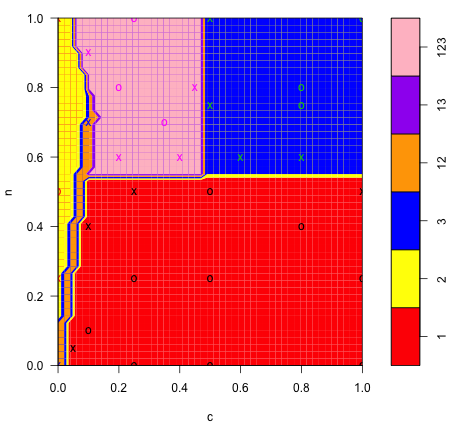
\includegraphics[width = 0.9 \linewidth]{Diagrams/basanta_phase-cropped}
\caption{Parameter regimes in spatial Glioblastoma game for $k = 0.5$. The numbers 1, 2, and 3 correspond to AG, INV, and GLY respectively. Multiple numbers indicate coexistence}
\end{figure}

\begin{figure}[H]
\centering
\begin{subfigure}[b]{0.4 \textwidth}
	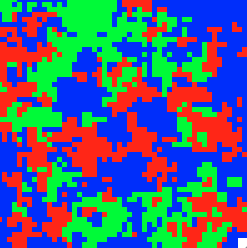
\includegraphics[width = 0.9 \textwidth]{Diagrams/Basanta/sample}
	\caption{Sample Output. Cells of type AG are red, INV green and GLY blue.}
\end{subfigure}
~
\begin{subfigure}[b]{0.4 \linewidth}
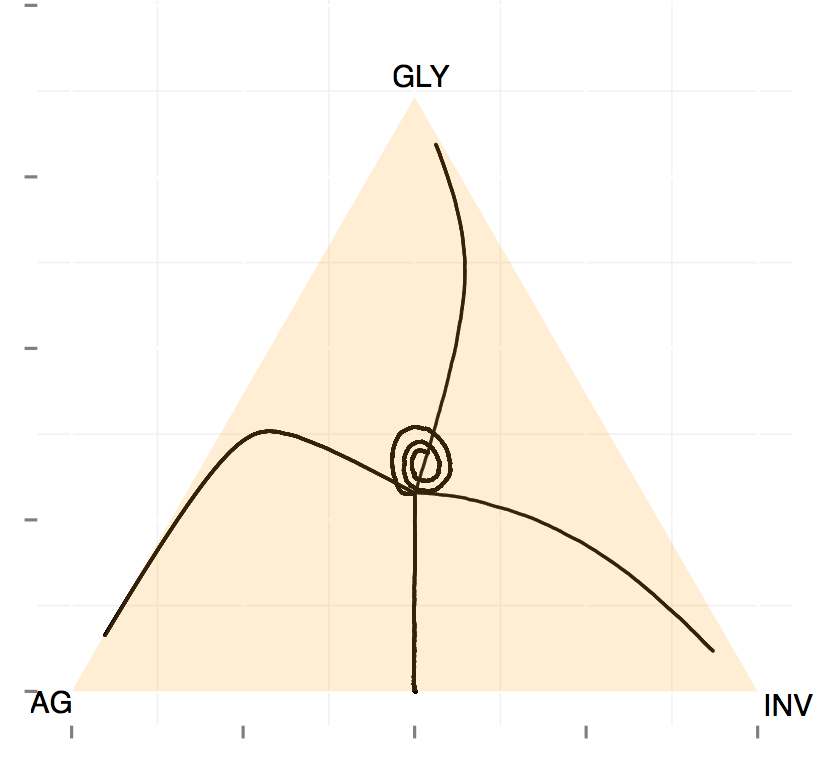
\includegraphics[width = 0.9 \linewidth]{Diagrams/basanta_trajectories}
\caption{Some sample trajectories plotted on the simplex. We have AG on the bottom left, INV on the right, and GLY on the top. }
\end{subfigure}
\end{figure}
  	

Based on simulation, the spatial model retains many of the features of the ODE model. Ignoring all behavior except coexistence or lack thereof, we can create a phase diagram. Since simulation is prohibitively time-consuming, we can use a Support Vector Machine to draw boundaries based on limited data. The output of the model is not very noisy, and we expect to have few mis-labelled points, we impose a very strict cost for misclassification when training the model.

 Based on the results for two species competition, we expected that the introduction of spatial consideration will be like a change in the game matrix -- potentially altering the critical values of the parameters. For example, at $c = 0.5$, there is a transition from all 3 types coexisting to GLY dominating, as predicted. Another common feature is that for $n > k$, GLY dominates AG.  The equilibrium of INV and GLY is uncommon, as for $k = 0.5$, it is sufficient that $n$ is positive for AG to be able to invade this equilibrium. The only point where this occurs with some regularity is near $(n,c) = (0,0)$. When $n$ and $c$ are zero, AG and INV beat on GLY. When GLY is dead, their respective interaction terms are zero, so they coexist. The other orange region may be an artifact that will disappear with further trials.

One important difference is that coexistence seems to be possible for a wider range of constraints. The constraint $k < \frac{cn}{1-c}$ implies that we need 
$$n > \frac{1}{2c} - \frac{1}{2}$$
This yields a value of $n > 1$ for $c < \frac{1}{3}$, but the spatial model permits coexistence in this parameter regime. This is consistent with others' work on stochastic spatial models in biology and economics, especially in the prisoner's dilemma\cite{Durrett2009}. 

We can plot some trajectories on the simplex to get a feel for how the frequencies evolve in time. The frequencies seem to approach their goal asymptotically, without executing a random walk on the simplex. The stable fixed point is interesting, as we can see the frequencies spiral into the center. It would be interesting to compare these flows to that of the mean-field ODE model in future work.  

\section*{Case 2: Multiple Myeloma}
In a 2009 paper, Dingli applies EGT to multiple myeloma evolution \cite{Dingli2009}. Multiple myeloma (MM) cells interact with the body's osteoclast (OC) and osteoblast(OB)cells, which are important in normal bone remodelling. When there are no MM cells, there is a stable equilibrium between OC and OB cells. MM cells promote the growth of OC cells by secreting osteoclast activating factors (OAF's) like interleukin  1$\beta$, RANKL, and MIP-1$\alpha$. MM cells also hinder OB differentiation by secreting Dickkopf-1 \cite{Dingli2009}. OC cells produce IL-6 and osteopontin to promote MM growth. The frequency-dependent interactions of the three cell types can be treated as an evolutionary game with a payoff matrix encapsulating the above information. Dingli further assumes that interactions between cells of the same type incur no cost or benefit. We can write the following payoff matrix, which captures the result of these interactions. 

$$A = \bordermatrix{\text{}&OC&OB&MM\cr
                OC& 0 & a& b \cr
                OB& e  &  0 & -d \cr
                MM& c & 0 & 0 \cr
               }$$

Dingli reduces the above matrix, $A$, to the minimal matrix, $B$, through the projective transformation $B_{ij} = \frac{A_{ij}}{\phi_j}$ where 
$\phi = {\begin{pmatrix} e & a & \frac{be}{c} \end{pmatrix}}$.
This yields the minimal matrix
$B = {\begin{pmatrix}
0 & 1 & \beta \\
1 & 0 & -\delta \\
\beta & 0 & 0
\end{pmatrix}}$. 
The projective transformation moves any internal fixed point into the barycenter of the simplex without changing the replicator dynamics or stability \cite{Hofbauer1998}. The dynamics can be divided into three regimes. For $\beta < 1$ and $\beta + \delta < 1$, an equilibrium between OC and OB is a globally attracting fixed point. For $\beta > 1$, an OC-MM equilibrium is globally attracting. Finally, for $\beta < 1$ and $\beta + \delta < 1$, we have bistability between an OB-OC equilibrium and an OC-MM equilibrium. 


\begin{figure}[htb]
\centering
\begin{subfigure}[b]{0.4 \textwidth}
\caption{Phase Portrait for  $\beta < 1$ and $\beta + \delta < 1$  }
\centering
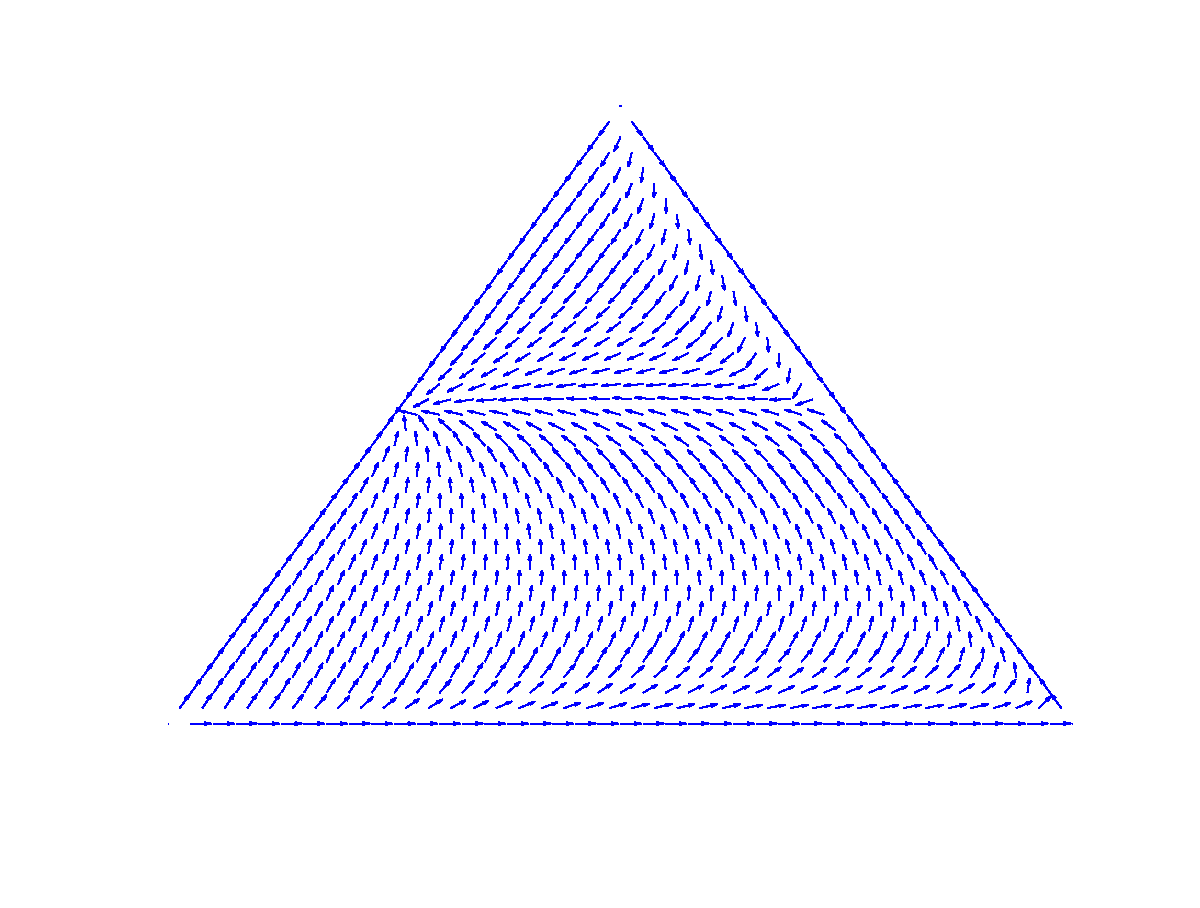
\includegraphics[width = 0.9 \textwidth]{Diagrams/Dingli/OCOB}
\end{subfigure}

\begin{subfigure}[b]{0.4 \textwidth}
\caption{Sample Phase Portrait for  $\beta < 1$ and $\beta + \delta > 1$  }
\centering
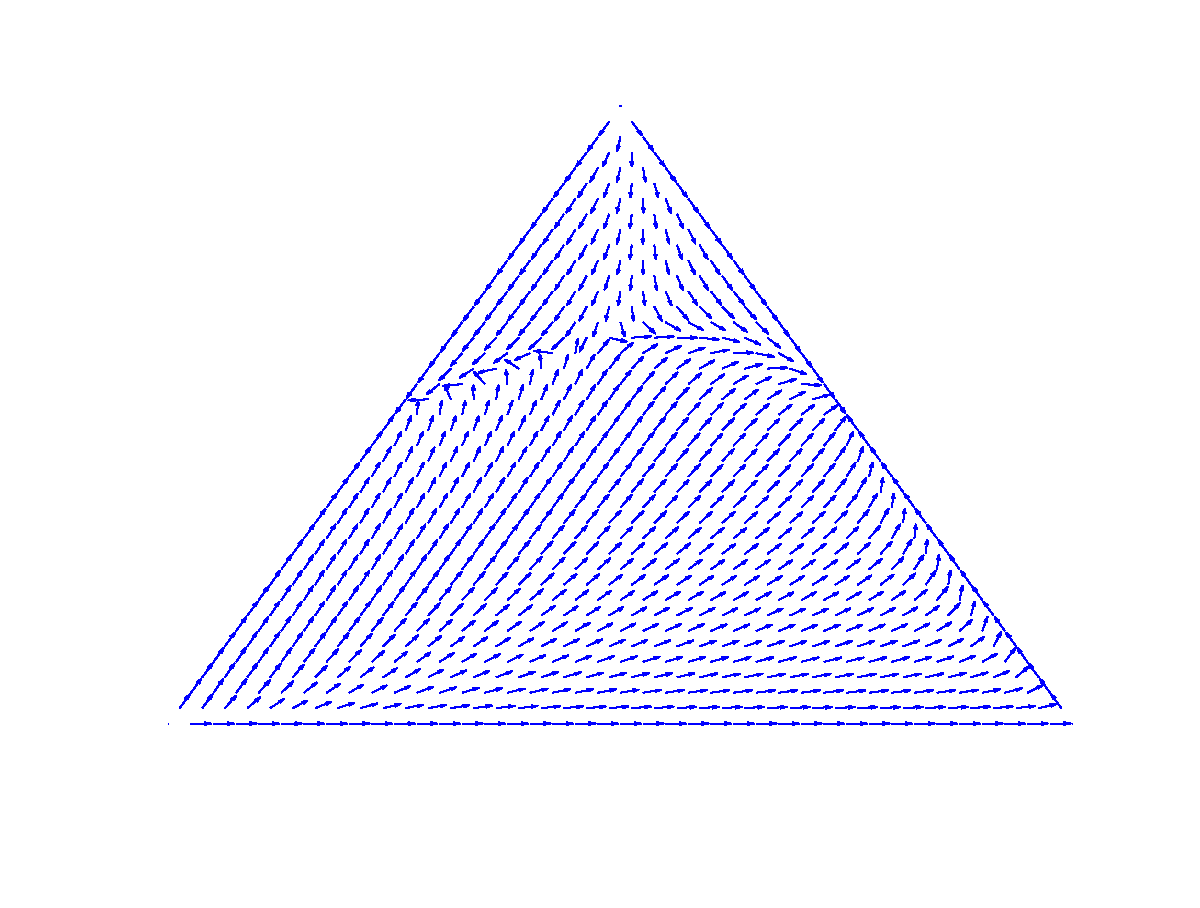
\includegraphics[width = 0.9 \textwidth]{Diagrams/Dingli/bistable}
\end{subfigure}
~
\begin{subfigure}[b]{0.4 \textwidth}
\caption{Sample Phase Portrait for  $\beta > 1$}
\centering
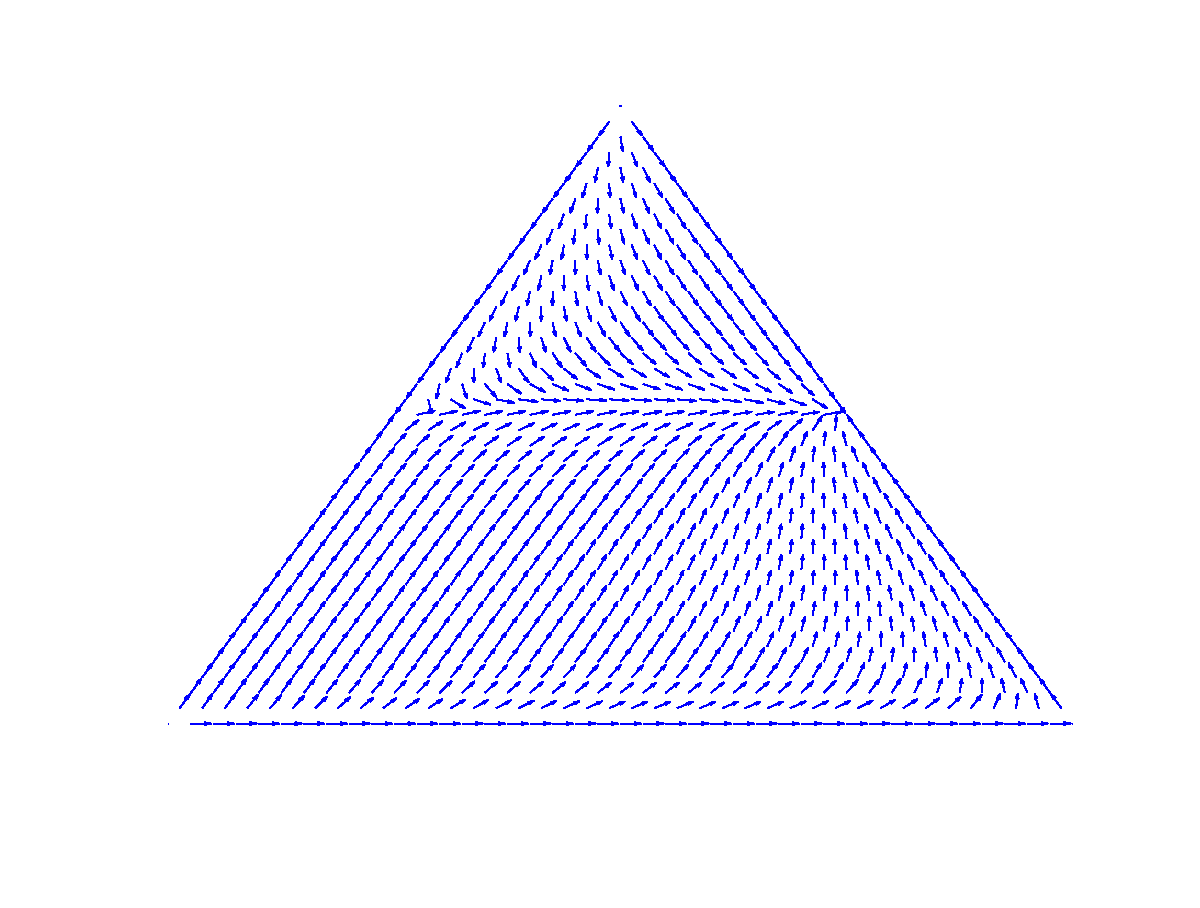
\includegraphics[width = 0.9 \textwidth]{Diagrams/Dingli/OCMM}
\end{subfigure}

\caption{Mean Field Phase Portraits}
\end{figure}

\begin{figure}[H]
\centering
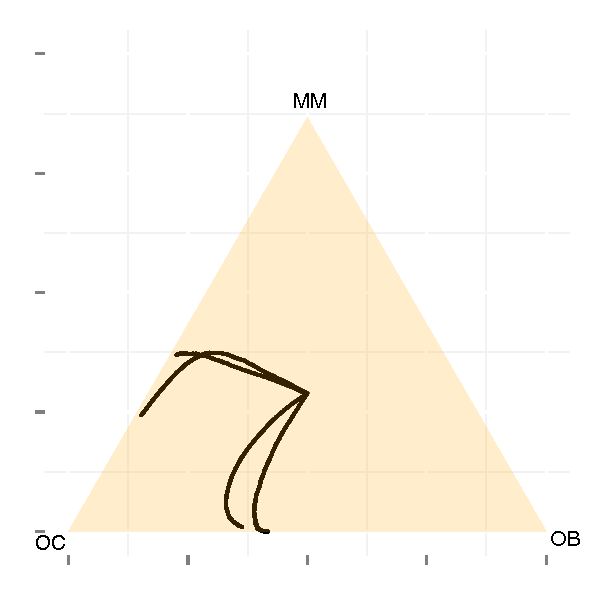
\includegraphics[width = 0.4 \linewidth]{Diagrams/dingli_trajectories}
\caption{Sample trajectories for each attracting basin from the spatial model}
\end{figure}
In the spatial case, things look different, mainly because of the absence of bi-stability. Instead, for each $\beta < 1$, there is a critical $\delta$ at which the equilibrium shifts from OC-OB to OC-MM.  

\pagebreak

\begin{figure}[!h]
\centering
\textbf{Phase Diagram}
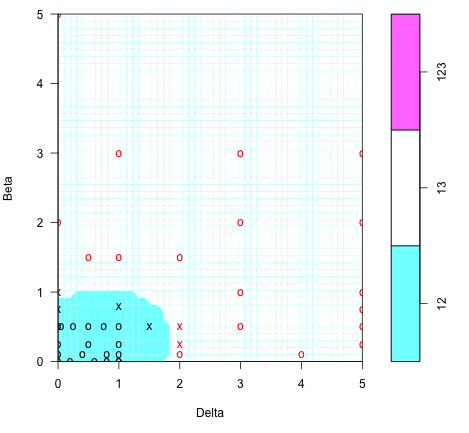
\includegraphics[width = 0.8 \linewidth]{Diagrams/dingli_phase-cropped}
\caption{Parameter regimes in spatial Myeloma Game. The numbers 1, 2, and 3 correspond to OC, OB, and MM respectively. Two numbers together indicate coexistence}
\end{figure}

\section*{Case 3: Toxin Game}
Tomlinson and Bodmer \cite{TomBod}1 consider the following example, where one cell produces a toxin that harms other tumor cells -- receiving a payoff. 

We have three types of cells
\begin{enumerate}
\item Producers (P) secrete a toxin
\item Resistant (R) cells to the above toxin
\item Baseline (B) cells neither produce nor resist the toxin
\end{enumerate}

We have the following interaction terms. All terms are assumed to be positive.
\begin{itemize}
\item $z$ : Baseline fitness
\item $e$ : Cost of producing toxin
\item $g$ :  Payoff of poisoning another cell. We have $g > e$, as the toxin would otherwise not be produced.
\item $h$ :  Cost of resisting the toxin
\item $f$ : Effect of toxin on non-resistant cells
\end{itemize}


We have the payoff matrix, 

$$A = \bordermatrix{\text{}& P & R & B\cr
                P & z - e - f + g & z - e & z - e + g \cr
                R & z - h  &  z - h & z - h \cr
                B & z - f & z & z \cr
               }$$

We add constants to each column to set the diagonals to 0.  Then, we have the reduced matrix


$$ A = \begin{pmatrix}
0 & h - e& g - e \\
f - k - h & 0 & -h \\
e - g& h & 0
\end{pmatrix} $$

As before, we can consider the pairwise interaction of each cell pair. \\

\textbf{1. R vs. B} B dominates R since $h > 0$ \\

\textbf{2. P vs. B} P dominates B since $k > 0$ \\

\textbf{3. P vs. R} \\
Here, the picture is more interesting. 
\begin{enumerate}
	\item $h > e$ : 
	\begin{enumerate}
		\item $h - e > f - g$ : P dominates R
		\item $h - e < f - g$ : We have a stable fixed point at 
		$$(p_P, p_R) = (\frac{h - e}{f-g}, \frac{e + f - g- h}{f -g})$$ 
		
		 Now we need to check if this equilibrium is invadable by B. If the fitness of type 3 is greater near the equilibrium, the equilbrium is invadable. Note that $f - g > 0$
		\begin{gather*}
		F_1 = F_2 = \frac{(h - e)(e + f  - g - h)}{f - g} \\
		F_3 = \frac{h- e}{f-g} (e - g) + \frac{e + f - g - h}{f - g} h \\
		F_3 - F_1 > 0 \rightarrow \\
		- g h - ef > 0 \\
		\frac{e}{g} > \frac{h}{f}
		\end{gather*}
		
		\begin{enumerate}
			\item $\frac{e}{g} > \frac{h}{f}$ : The P-R equilibrium is invadable. An interior fixed point is attracting and globally stable.
			\item  $\frac{e}{g} < \frac{h}{f}$ : The P-R equilibrium is attracting.
		\end{enumerate}
	\end{enumerate}
	\item $h < e$
	\begin{enumerate}
		\item $h - e > f -g$  : unstable fixed point on P-R boundary. P dominates.
		\item $h - e < f - g$ : R dominates P, leading to a cyclic competition
	\end{enumerate}
\end{enumerate}




The simulation results look strange, so I am still working them out. I will include them at a later time. 



\chapter*{Conclusion}
We have created a stochastic spatial model for a generic evolutionary game and applied it to the interplay of phenotypes in tumor growth. The interacting particle system retains many of the important dynamical features of the mean-field approximation, including certain critical phase transition values. The spatial structure encouraged coexistence in one game with a stable fixed point, making it possible for a wider range of parameters. In bi-stable systems, we can observe a phase transition that depends on the parameters, in lieu of actual bi-stability. Tumors are famously heterogeneous, with multiple cell types in complex spatial arrangements. \\

Spatial considerations can change the qualitative features of an evolutionary game, explaining this coexistence better than a simpler mean-field approach. A game-theoretic approach could offer clinical insights into the relationship between cancerous phenotypes. Targeting specific phenotypes can have counterintuitive effects on the tumor as a whole. New methods of treatment could attempt to change the parameters of this evolutionary game, enabling the tumor to select malignant phenotypes out on its own.\\

For future work, it would be interesting to look at the mean-field ODE more closely, specifically the Eigenvalues and Eigenvectors of the given fixed points. It is possible that this could shed light on time-evolution of the spatial game. One might also look more closely at the analytical results for 2-strategy games, to see if an updated game matrix can accurately predict equilibrium frequencies in the full spatial model. 



\newpage \bibliographystyle{plain}
\bibliography{bibliog}

\end{document}


\comment{
In the spatial treatment, phase portraits with a globally attracting equilibrium should result in coexistence between the relevant types \cite{Durrett2009}. Indeed, phase portraits with OB-OC or OC-MM equilibria result in the same outcome for the spatial case. For $\beta < 1$ and $\beta + \delta > 1$, the replicator equation suggests that the location of the initial condition with respect to the saddle point should determine which basin of attraction the system falls into. 
Our model shows that for each $\beta$, there is a critical $\delta$ at which the system switches from an OC-OB equilibrium to an OC-MM equilibrium. In addition, there is a critical $\beta$ below which we will always have an OC-OB equilibrium for any choice of $\delta$.
}


\comment{
\begin{figure}[htb]
\caption{Sample output for $\beta < 1$ and $\beta + \delta > 1$}
\centering
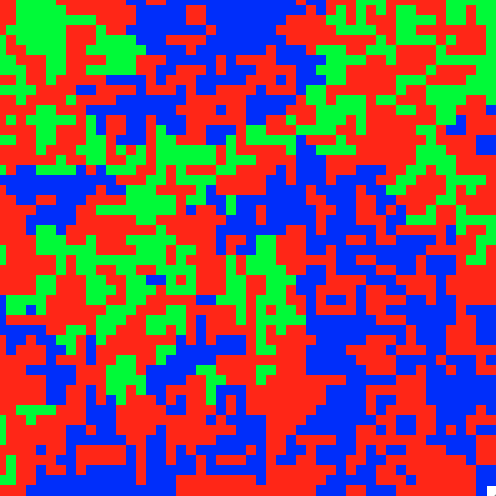
\includegraphics[width = 1.5 in]{Diagrams/Dingli/sample}
\end{figure}

\begin{figure}[htb]
\caption{For each $\beta$, there is a critical $\delta$ below which OB always wins. There is also a critical $\beta$ (0.35) below which there is no $\delta$ for which MM wins.}
\centering
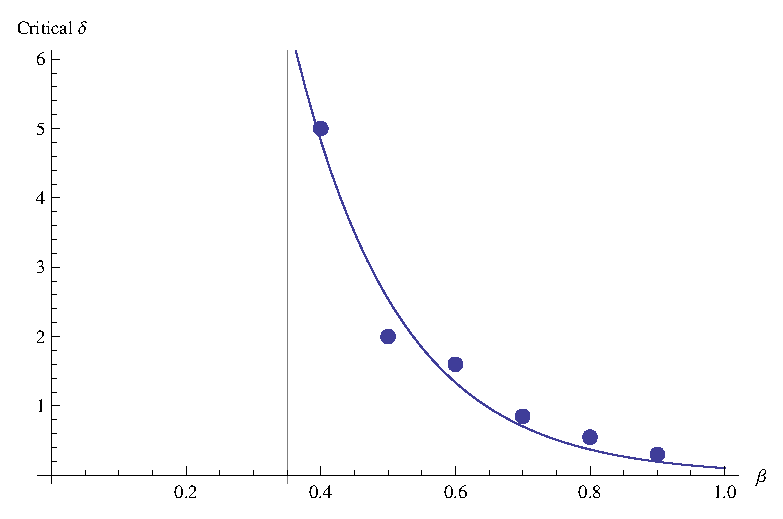
\includegraphics[width = 1.5 in]{Diagrams/Dingli/critdeltavsbeta}
\end{figure}
}







		